Ionospheric perturbations also can take place due to space weather and geomagnetic storms. So, in order to discard such events we investigated the space weather in the day each event occurred. We investigated the solar wind conditions in the event day and the previous 7 days, the x-ray flux %the planetary K index (Kp index) at the event day and the previous two days 
and the Dst index at the event date.   

%\subsection{Planetary K index}

 %In figure \ref{fig:Kp-index} we show the Kp index for the day of the Caribbean bolide event. We discarded events whose Kp index is equal or grater than 4 at the day and time the meteor passage occured. These data were obtained from the NOAA/Space Weather Prediction Center. We found that the Kp index is lower than 4 for the event date and adjacent days, so we can safely assume that geomagnetic storms are not a treat for our detection of TIDs. 

%\begin{figure}
%\centering
%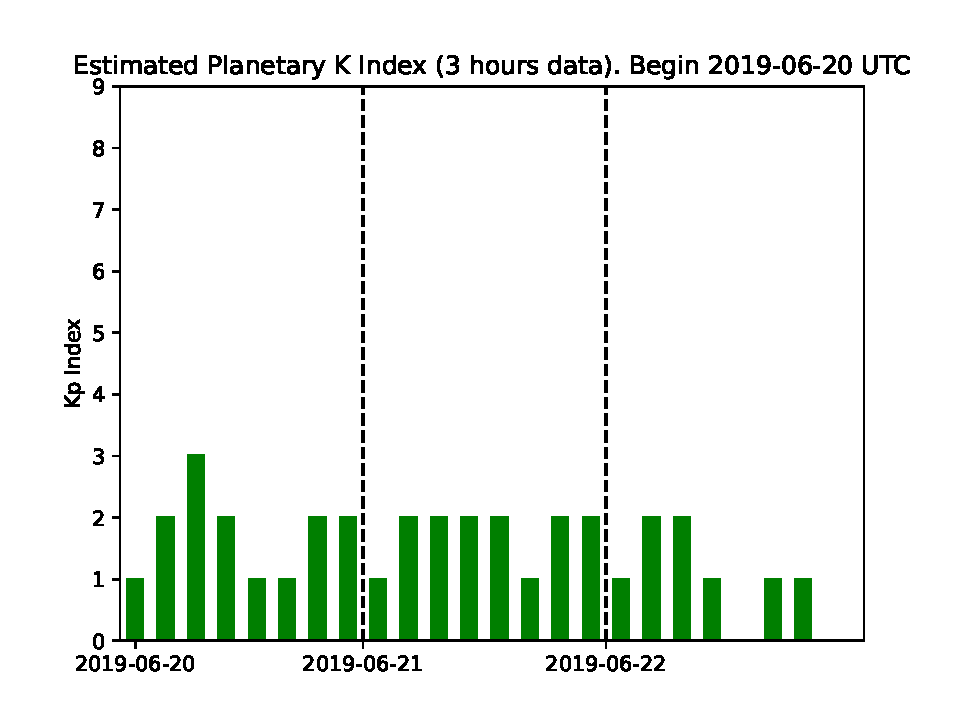
\includegraphics[width=\linewidth]{./figures/2019-06-22 Kp index}
%\caption{Planetary K index for 2019-06-22 and two previous days (NOAA/Space Weather Prediction Center). Only Moderate K index warnings were issued.}
%\label{fig:Kp-index}
%\end{figure}

\subsection{Dst Index}

We obtained measurements of Dst Index from WDC for Geomagnetism, Kyoto DST index service (\url{https://wdc.kugi.kyoto-u.ac.jp/dstdir/}), and is shown in figure \ref{fig:Dst_index}. We see that  Dst index remains practically constant around zero, which confirms that there were not geomagnetic storms that could prevent us from detecting TIDs in our GPS data.

\subsection{Solar wind}

Another source of ``space weather noise'' that we should discard is unusual solar wind behavior or even coronal mass ejections. We collected data from the Deep Space Climate Observatory (DSCOVR) of solar wind speed, temperature, density, dynamic pressure and solar magnetic field, in order to monitor the solar wind behavior in the day of the event and the previous 6 or 7 days.% In figure \ref{fig:wind_temp} we can see in the event day and the prior week solar wind temperature remained between $\sim \SI{1e4}{}$ and $\sim \SI{1e5}{K}$. %Solar magnetic field in the range of $\sim -6$ to $\sim \SI{6}{nT}$, while total magnetic field did not go over \SI{10}{nT}. 
%Neither for temperature or magnetic field detected sudden changes of magnitude. 

We were concerned of shock waves produced by rapid wind reaching slow wind, which also may produce TIDs and thus contaminating our GPS data, and may not be distinguishable from TIDs produced by the meteor passage. To check the presence of such shock waves, we estimate the relative velocity of solar wind of one day respect the previous one. The results are shown in figure \ref{fig:solar-relative-speed}, where we see that this velocity is almost constant and gives no chance for a fast stream reaching a slow one producing a shock wave. 

\begin{figure*}
    \centering
    \begin{adjustwidth}{-\extralength}{0cm}
    \includegraphics[width=\linewidth]{../figures/caribbean-Dst-index.pdf}
    \end{adjustwidth}
    \caption{Dst index for 2019 June 22th. Data obtained from WDC for Geomagnetism, Kyoto DST index service.}
    \label{fig:Dst_index}
\end{figure*}

%\begin{figure}
%    \centering
%    \includegraphics[width=\linewidth]{figures/solar-wind-temperature-all.pdf}
%    \caption{Solar wind temperature in logarithmic scale from 2019-06-16 to event date. Each curve represent one day data.}
%    \label{fig:wind_temp}
%\end{figure}

%\begin{figure*}
%    \centering
%    \includegraphics[width=\linewidth]{figures/solar-magnetic-field-all.pdf}
%    \caption{Solar magnetic field components (colors) and total magnetic field (black) for the event date and the prior week. Each curve represent one day data.}
%    \label{fig:solar_mag_field}
%\end{figure*}

\begin{figure*}
    \centering
    \begin{adjustwidth}{-\extralength}{0cm}
    \includegraphics[width=\linewidth]{../figures/solar_speed_all_wcs.pdf}
    \end{adjustwidth}
    \caption{Relative speed of solar wind at the event day and previous week respect the previous day, normalized with speed of sound. Each curve represents one day data.}
    \label{fig:solar-relative-speed}
\end{figure*}

\subsection{X-rays flux}

X rays are a clear source of ionization, they are generated mainly in the corona due to magnetospheric activity. A sudden increase of the flux or sudden variations may be a source of GW or giving appearance of GW. We investigated the X ray flux from the Sun at the event date and the previous week and collected data from the NOAA Space Prediction Center. %We show the results in figures \ref{fig:X-rays-1} to . 
X-rays flux remained constant in the time range we collected data.

%\begin{figure}
%    \centering
%    \includegraphics[width=\linewidth]{figures/20190618_xray.jpg}
%    \caption{X-ray flux obtained from NOAA Space Prediction Center, starting at Jun 16 00:00 hrs UT and ending at Jun 19 24:00 hrs UT. Color curves represent data from GOES satellites and the wavelength range: purple for GOES 14 in the range from 0.5 to \SI{4.0}{\AA}, yellow for GOES 14 in the range from 1.0 to \SI{8.0}{\AA}, blue for GOES 15 in the range from 0.5 to \SI{4.0}{\AA} and red for GOES 15 in the range from 0.5 to \SI{4.0}{\AA}. In all cases the X-ray flux remains constant.}
%    \label{fig:X-rays-1}
%\end{figure}

%\begin{figure}
%    \centering
%    \includegraphics[width=\linewidth]{figures/20190621_xray.jpg}
%    \caption{Same as figure \ref{fig:X-rays-1} but data starts at Jun 19 00:00 hrs and ends at Jun 21 24:00 hrs.}
%    \label{fig:X-rays-2}
%\end{figure}

%\begin{figure}
%    \centering
%    \includegraphics[width=\linewidth]{figures/20190622_xray.jpg}
%    \caption{Same as figures \ref{fig:X-rays-1} and \ref{fig:X-rays-2} but data starts at Jun 20 00:00 hrs and ends at Jun 22 24:00 hrs, which includes the event date.}
%    \label{fig:X-rays-3}
%\end{figure}

\subsection{dTEC and W index}

Finally we wanted to check the effects of solar cycle variations. The critical frequencies of reflection $f_c$ is proportional to the number of sunspots in the Sun, thus affecting our TEC measurements. Seasonal variations may be important too, since solar flux varies as the Earth revolves around the Sun. To measure these effects, we computed dTEC, defined as \citep{Gulyaeva:2008}:

\begin{align}
    dTEC = \log_{10}\frac{TEC}{medTEC}
\end{align}

Where $TEC$ is the average TEC measurements of a certain day, while $medTEC$ is the median TEC of the 27 previous days, corresponding to the solar rotation period. dTEC was computed for the event day with each station. The W index reveals TEC behavior and the ionospheric perturbation level. In table \ref{tab:W-index} we show the W index levels, the corresponding dTEC and how perturbed is the ionosphere. %In this case and nearby stations, we noted that meteor fragmentation occurred briefly before local sunset, so solar terminator effects must be accomplished.

\begin{table}
    \centering
    \caption{W index values with their corresponding dTEC values and a brief description of the ionospheric state when those index is obtained \citep{Gulyaeva:2008}.}
    \begin{tabular}{lcr}\toprule
    dTEC & W index   & Ionospheric state     \\
    \hline
    $dTEC = 0$ & 0   & Reference quiet state \\
    $0<|dTEC|<0.046$ & $\pm 1$ & Quiet state \\
    $0.046<|dTEC|<0.155$ & $\pm 2$ & Weak perturbation \\
    $0.155<|dTEC|<0.301$ & $\pm 3$ & Moderated storm   \\
    $|dTEC|> 0.301$  & $\pm 4$ & Intense storm         \\\bottomrule
    \end{tabular}
    \label{tab:W-index}
\end{table}

We estimated the dTEC and the corresponding W index for all the GPS stations from we collected data. An example is shown in figure \ref{fig:dtec-boav}. In this figure we see how dTEC changes in time on the meteor date. The moment the meteor fragmented is shown with a black dashed line. The W index values are shown as the colored background.

\begin{figure}
    \centering
    \begin{adjustwidth}{-\extralength}{0cm}
    \includegraphics[width=\linewidth]{../figures/dTEC_Windex_boav.pdf}
    \end{adjustwidth}
    \caption{dTEC and W index for station BOAV. dTEC is shown as the continuous blue curve. The corresponding W index ranges are shown as the colored backgrounds, from quiet state in blue to strong storm $(|W|=4)$ in red. The meteor fragmentation time is shown in vertical dashed line, and  as additional information the local sunrise and sunset in dashed blue lines.}
    \label{fig:dtec-boav}
\end{figure}

In this example and most of the stations we noted that the W index stands in negative values from -2 to -3 and normalizes to 1 after the 10 hrs. To understand the origin of this behavior we also included the local sunrise and sunset, and we found out that W index is quite negative at night, and normalizes after sunrise (local night occurs from 21-23 hrs of previous day to $\sim \SI{10}{hrs}$, check table \ref{tab:table-stations} for accurate information). Also found out that meteor fragmentation occurred a few hours before sunset, depending on the station. The high fluctuations in the dTEC may be attributable to the fact that at nighttime the logarithm is more susceptible to small variations since TEC is closer to zero. Fluctuations normalize after sunrise.

\subsection{Solar terminator}

If a meteoroid passage and explosion occurs at sunrise or sunset, the passage of the solar terminator should be taken into account since is one of the GW sources and cause some disturbances in the ionosphere \citep{Somsikov:2011}. In figure \ref{fig:solar_terminator} we see that meteor fragmentation occurred outside the solar terminator, but some GPS stations (KOUG and KOUR) are located very close to (sunset comes about 20 minutes after the fragmentation). In order to distinguish between the effects of the meteor and the solar terminator we detrended GPS data for the mentioned stations at dates prior of the meteor fall, those dates are close enough to guarantee that the sunset occurs almost at the same time. With this we can isolate the effects of the solar terminator and analyze its effects to check how they affect into our time series. Some results are shown in figure \ref{fig:solar_terminator_time_series} for station KOUG, PRNs 2 and 12. In these cases we see that the solar terminator does perturb the ionosphere, and its effects can bypass the detrending process, since they consist in wave-like variations of TEC. But these perturbations most of the time are weaker and distinguishable from the perturbations produced by the meteor passage, so we can safely assume that they don't affect in our detections. Even more, comparing time series from previous days we can help us to discriminate between time series with detected TID from others where only noise is recorded since some patterns in the time series can be detected. Time series too similar with the previous days can be classified as non detections.

\begin{figure}
    \centering
    \begin{adjustwidth}{-\extralength}{0cm}
    \includegraphics[width=\linewidth]{../figures/BOAV-KOUG-KOUR-sunset.png}
    \end{adjustwidth}
    \caption{Solar terminator position for the most southern stations: BOAV (yellow shadow), KOUG and KOUR (gray shadow). The corresponding sunset times are labeled in the corresponding terminator line, and the sunset time difference between KOUG and KOUR stations is just 2 minutes. Sunset time in stations KOUR and KOUG occured 20 minutes later than meteor fragmentation.}
    \label{fig:solar_terminator}
\end{figure}

\begin{figure*}
    \centering
    \begin{adjustwidth}{-\extralength}{0cm}
    \begin{tabular}{ccc}
    \includegraphics[width=0.33\linewidth]{../figures/KOUG_2019-06-19_PRN2.pdf} & \includegraphics[width=0.33\linewidth]{../figures/KOUG_2019-06-20_PRN2.pdf}& \includegraphics[width=0.33\linewidth]{../figures/koug-sTEC_series_PRN_2.pdf} \\
    \includegraphics[width=0.33\linewidth]{../figures/KOUG_2019-06-19_PRN12.pdf} & \includegraphics[width=0.33\linewidth]{../figures/KOUG_2019-06-20_PRN12.pdf} & \includegraphics[width=0.33\linewidth]{../figures/koug-sTEC_series_PRN_12.pdf}
    \end{tabular}
    \end{adjustwidth}
    \caption{Detrended sTEC time series for station KOUG for the days 2019-06-19, 2019-06-20 and 2019-06-22 (three days before meteor fall, two days and the meteor fall date, from left to right). The satellite receiver LOS with PRN 2 is in top, and the LOS with PRN 12 is in bottom.}
    \label{fig:solar_terminator_time_series}
\end{figure*}

\subsection{sTEC time series}

We detrended the RINEX data we obtained for all stations and analyzed separately each satellite-receiver time series in order to find by visual inspection wave-like features. We must be careful when making conclusions about the presence of TIDs produced by the bolide in the cases when the sunset and the fragmentation occurred in a short period of time. We separated those time series where we detected the presence of such features (see \S \ref{ssec:Morlet}), from all the others, which could be too noisy, too few data, etc. A significant sample of about 10\% of all the time series we have are shown in figures \ref{fig:sTEC-series}-\ref{fig:sTEC-series3}.  

\begin{figure*}
    \centering
    \begin{adjustwidth}{-\extralength}{0cm}
    \begin{tabular}{cc}
    \includegraphics[width=0.45\linewidth]{../figures/cn04-sTEC_series_PRN_6-previous.pdf}  \includegraphics[width=0.45\linewidth]{../figures/cn04-sTEC_series_PRN_6.pdf}\\
    \includegraphics[width=0.45\linewidth]{../figures/cn40-sTEC_series_PRN_12-previous.pdf}  \includegraphics[width=0.45\linewidth]{../figures/cn40-sTEC_series_PRN_12.pdf}\\
    \includegraphics[width=0.45\linewidth]{../figures/ttsf-sTEC_series_PRN_2-previous.pdf}  \includegraphics[width=0.45\linewidth]{../figures/ttsf-sTEC_series_PRN_2.pdf}\\
%    \includegraphics[width=0.3\linewidth]{}  \includegraphics[width=0.3\linewidth]{}\\
    \end{tabular}
    \end{adjustwidth}
    \caption{sTEC time series for stations where TIDs are likely to be detected. In the left panels we show the time series for the previous day of meteor fall, and in the right panels the time series for the meteor fall date.}
    \label{fig:sTEC-series}
\end{figure*}

\begin{figure*}
    \centering
    \begin{adjustwidth}{-\extralength}{0cm}
    \begin{tabular}{cc}
    \includegraphics[width=0.45\linewidth]{../figures/ttuw-sTEC_series_PRN_2-previous.pdf}  \includegraphics[width=0.45\linewidth]{../figures/ttuw-sTEC_series_PRN_2.pdf}\\
    \includegraphics[width=0.45\linewidth]{../figures/boav-sTEC_series_PRN_2-previous.pdf}  \includegraphics[width=0.45\linewidth]{../figures/boav-sTEC_series_PRN_2.pdf}\\
    \includegraphics[width=0.45\linewidth]{../figures/boav-sTEC_series_PRN_12-previous.pdf}  \includegraphics[width=0.45\linewidth]{../figures/boav-sTEC_series_PRN_12.pdf}\\
    \end{tabular}
    \end{adjustwidth}
    \caption{Continuation of figure \ref{fig:sTEC-series}}
    \label{fig:sTEC-series2}
\end{figure*}

\begin{figure*}
    \centering
    \begin{adjustwidth}{-\extralength}{0cm}
    \begin{tabular}{cc}
    \includegraphics[width=0.45\linewidth]{../figures/koug-sTEC_series_PRN_2-previous.pdf} & \includegraphics[width=0.45\linewidth]{../figures/koug-sTEC_series_PRN_2.pdf}\\
    \includegraphics[width=0.45\linewidth]{../figures/koug-sTEC_series_PRN_12-previous.pdf} & \includegraphics[width=0.45\linewidth]{../figures/koug-sTEC_series_PRN_12.pdf}\\
    \includegraphics[width=0.45\linewidth]{../figures/gre1-sTEC_series_PRN_2-previous.pdf} & \includegraphics[width=0.45\linewidth]{../figures/gre1-sTEC_series_PRN_2.pdf}
    \end{tabular}
    \end{adjustwidth}
    \caption{Continuation of figures \ref{fig:sTEC-series} and \ref{fig:sTEC-series2}.}
    \label{fig:sTEC-series3}
\end{figure*}

In order to check which stations actually observed the TIDs generated by the bolide fragmentation, we proceeded to learn which stations were located near the bolide trajectory at the event time or the next few hours. Stations located far of the bolide trajectory are more likely to have detected other phenomena not related with the bolide passage. Since we are using sTEC measurements, we want to have a picture of the line of sight we are considering in our sTEC measurements. To do such task we will compare the bolide trajectory with all of the satellites in local coordinates (azimuth and elevation) to see if at least one was close enough to the bolide trajectory and its elevation. Such diagrams are shown in figures  for the same stations of figures \ref{fig:sTEC-series} - \ref{fig:sTEC-series3}. Ideally if the satellite trajectory intersects the meteor trajectory in our TEC series we see the TEC variations in the line of sight where the meteor passed. But is also possible that a slightly distant satellite detected some TIDs that propagated away from the source.

\begin{figure*}
\begin{adjustwidth}{-\extralength}{0cm}
    \begin{tabular}{cc}
      \includegraphics[width=0.45\linewidth]{../figures/azimuth-elevation-map-boav-polar-hlght.png}   & \includegraphics[width=0.45\linewidth]{../figures/azimuth-elevation-map-cn04-polar-hlght.png} \\
            \includegraphics[width=0.45\linewidth]{../figures/azimuth-elevation-map-cn40-polar-hlght.png}   & \includegraphics[width=0.45\linewidth]{../figures/azimuth-elevation-map-gre1-polar-hlght.png} \\
     \includegraphics[width=0.45\linewidth]{../figures/azimuth-elevation-map-koug-polar-hlght.png}   & \includegraphics[width=0.45\linewidth]{../figures/azimuth-elevation-map-ttsf-polar-hlght.png} \\
    \end{tabular}
    \end{adjustwidth}
    \caption{Azimuth-Elevation maps for GPS stations which presumably detected TIDs. In colored curves we show the satellites trajectories with their respective label, the trajectory starts at the big colored dot. The black dots are the meteor trajectory using the GLM data and the magenta dashed curve represent the meteor trajectory using the velocity parameters from table \ref{tab:Meteor-parameters}.}
    \label{fig:azimuth-elevations-maps-1}
\end{figure*}

\begin{figure*}
\begin{adjustwidth}{-\extralength}{0cm}
    \centering
    \begin{tabular}{cc}
    \includegraphics[width=0.5\linewidth]{../figures/boav_satellites_positions_terminator_21-25-48.png} & \includegraphics[width=0.5\linewidth]{../figures/cn04_satellites_positions_terminator_21-25-48.png}\\
    \includegraphics[width=0.5\linewidth]{../figures/cn40_satellites_positions_terminator_21-25-48.png} & \includegraphics[width=0.5\linewidth]{../figures/gre1_satellites_positions_terminator_21-25-48.png} %\\
   % \includegraphics[width=0.5\linewidth]{figures/koug_satellites_positions_terminator_21-25-48.png} & \includegraphics[width=0.5\linewidth]{figures/ttsf_satellites_positions_terminator_21-25-48.png}
    \end{tabular}
    \end{adjustwidth}
    \caption{Position of IPP in the satellite-receiver LoS for the same GPS stations as figure \ref{fig:azimuth-elevations-maps-1}. The GLM data are shown in magenta dots, the fragmentation position in a red star and the estimated trajectory from 1 hour before fragmentation to a few seconds after fragmentation is shown in green dashed line. The position of the GPS station is shown with a blue triangle. The solar terminator appears in BOAV and KOUG stations as a blue shadow.}
    \label{fig:satellites-and-terminator}
\end{figure*}
%The mathematical proccedure to change the GLM data and the estimated trajectory, using the parameters from table \ref{tab:Meteor-parameters}. 
%\subsection{Wavelet power spectrum}

%For each TEC series like figure \ref{fig:detrending-example} we computed $|W_n(s)|^2$ to find any wave-like features in any of the TEC series, where $s$ is the wavelet scale (somehow is the analogous to the wavelength). The presence of this features allow us to trace the TEC perturbations produced by the meteor. Examples are shown in figure \ref{fig:power-spectrums}. Due to the fact we are working with finite time series, edge effects become important at the beginning or the end of the time series, and when the wavelet scale is similar or greater than the time series length. The limit when these errors become important is called Cone of Influence (COI), the COI is shown as a white dashed line in figure \ref{fig:power-spectrums}. At a closer look of this spectra is clear that in some cases the wavelet spectra in the previous day is more intense than the event day. This happens because no TEC perturbations was really detected, but instead noise appears as wavelets. This is an indicator that the TEC perturbances either propagate to other location or it is too faint to be detectable.


%\begin{figure*}
%  \begin{tabular}{cc}
%  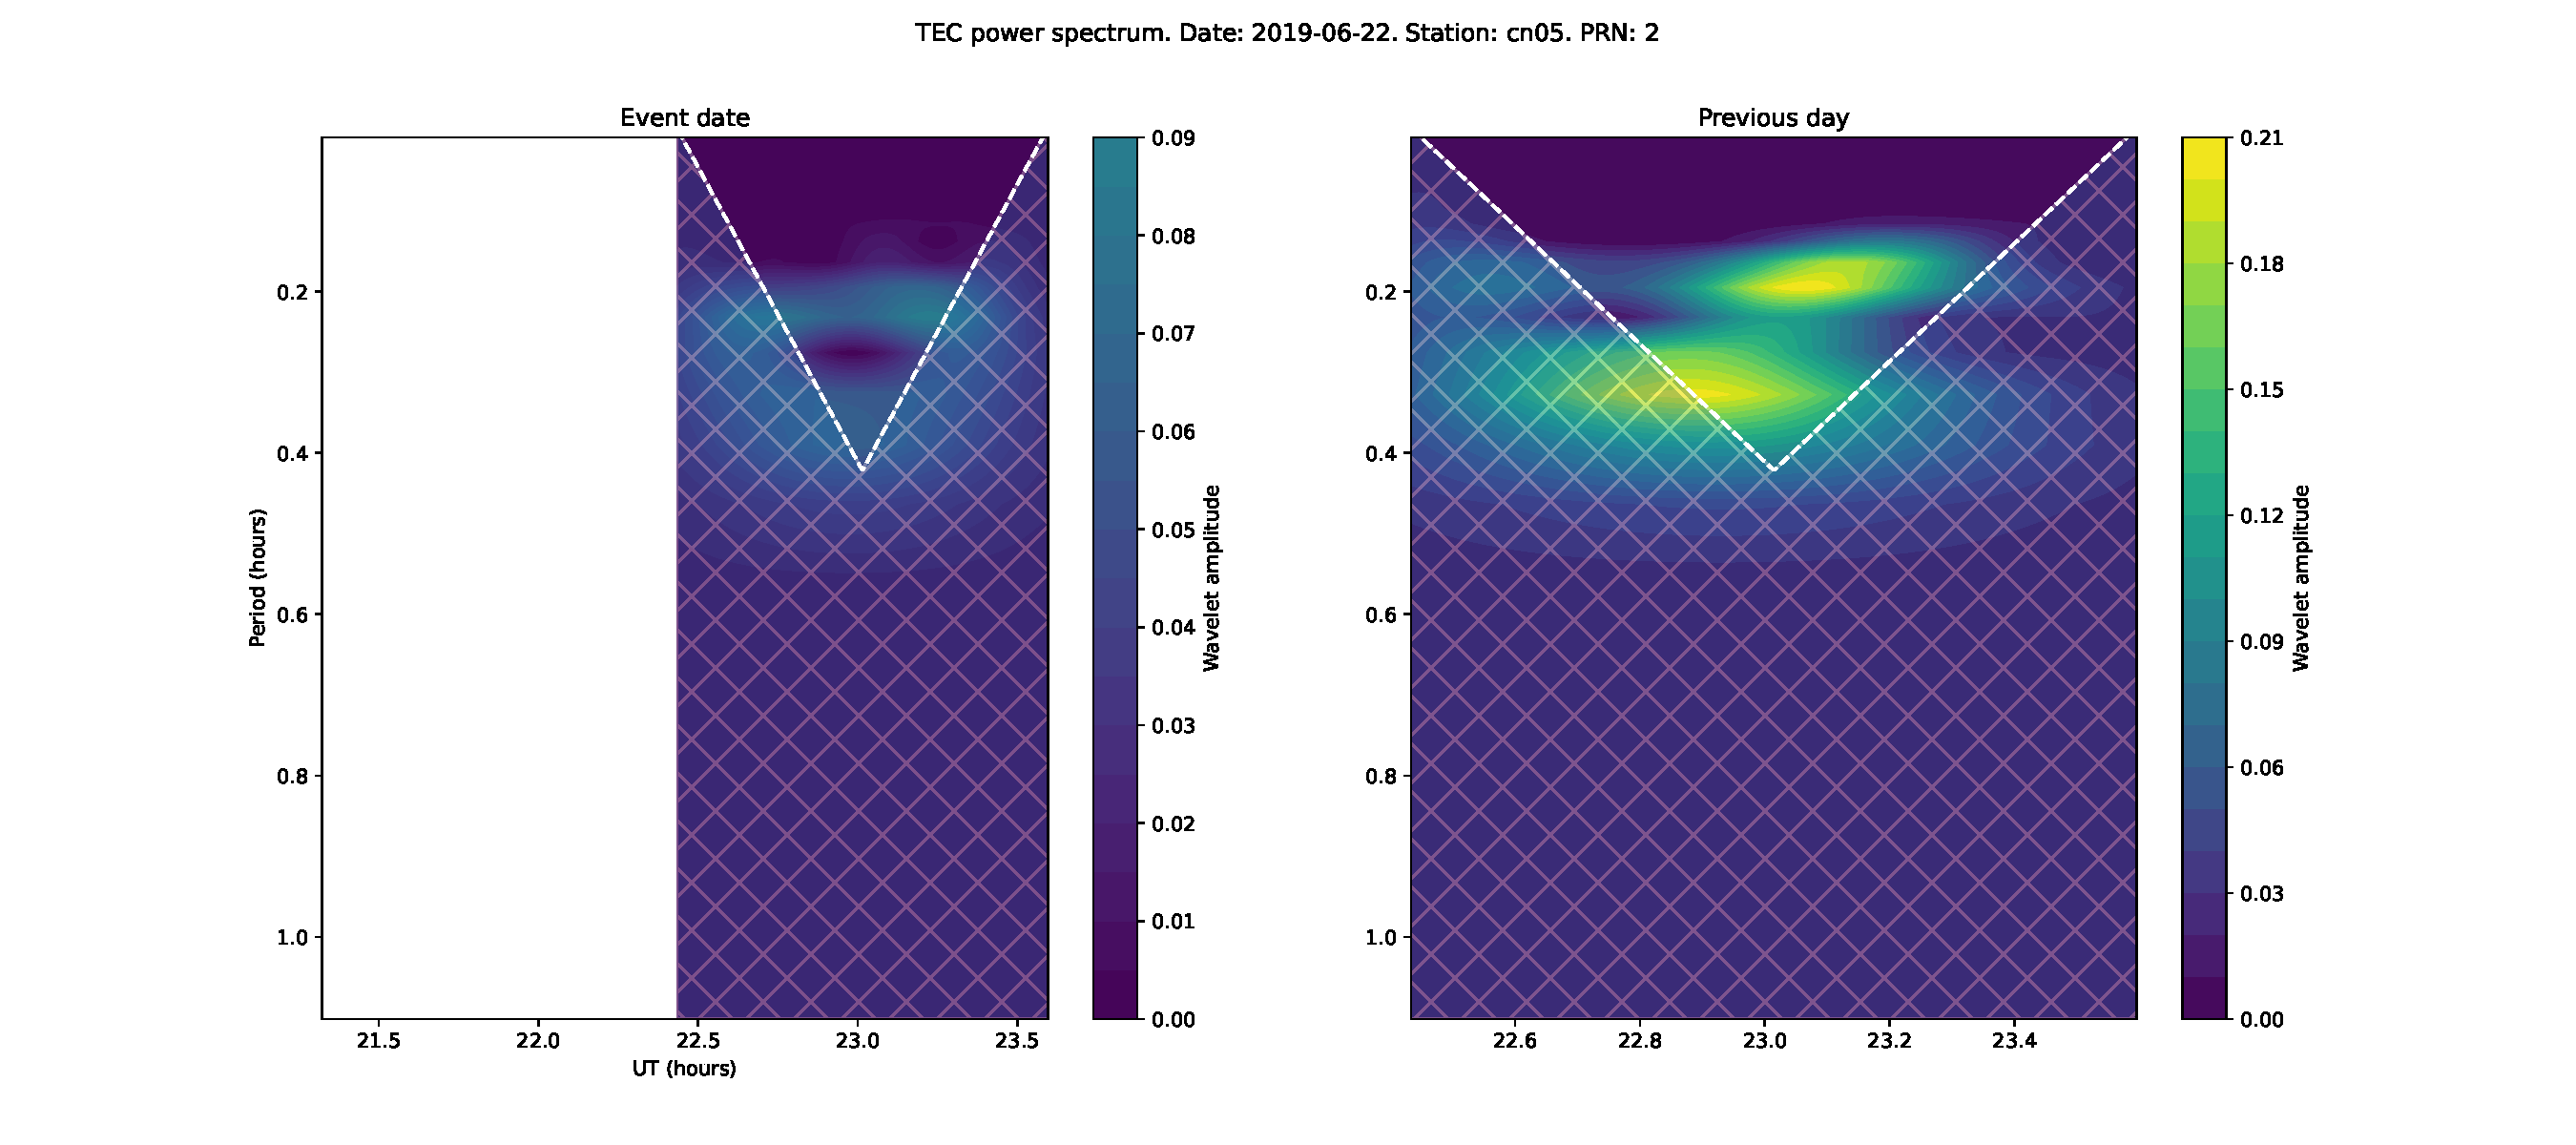
\includegraphics[width=0.5\linewidth]{./figures/cn05-PRN2-contour}  & %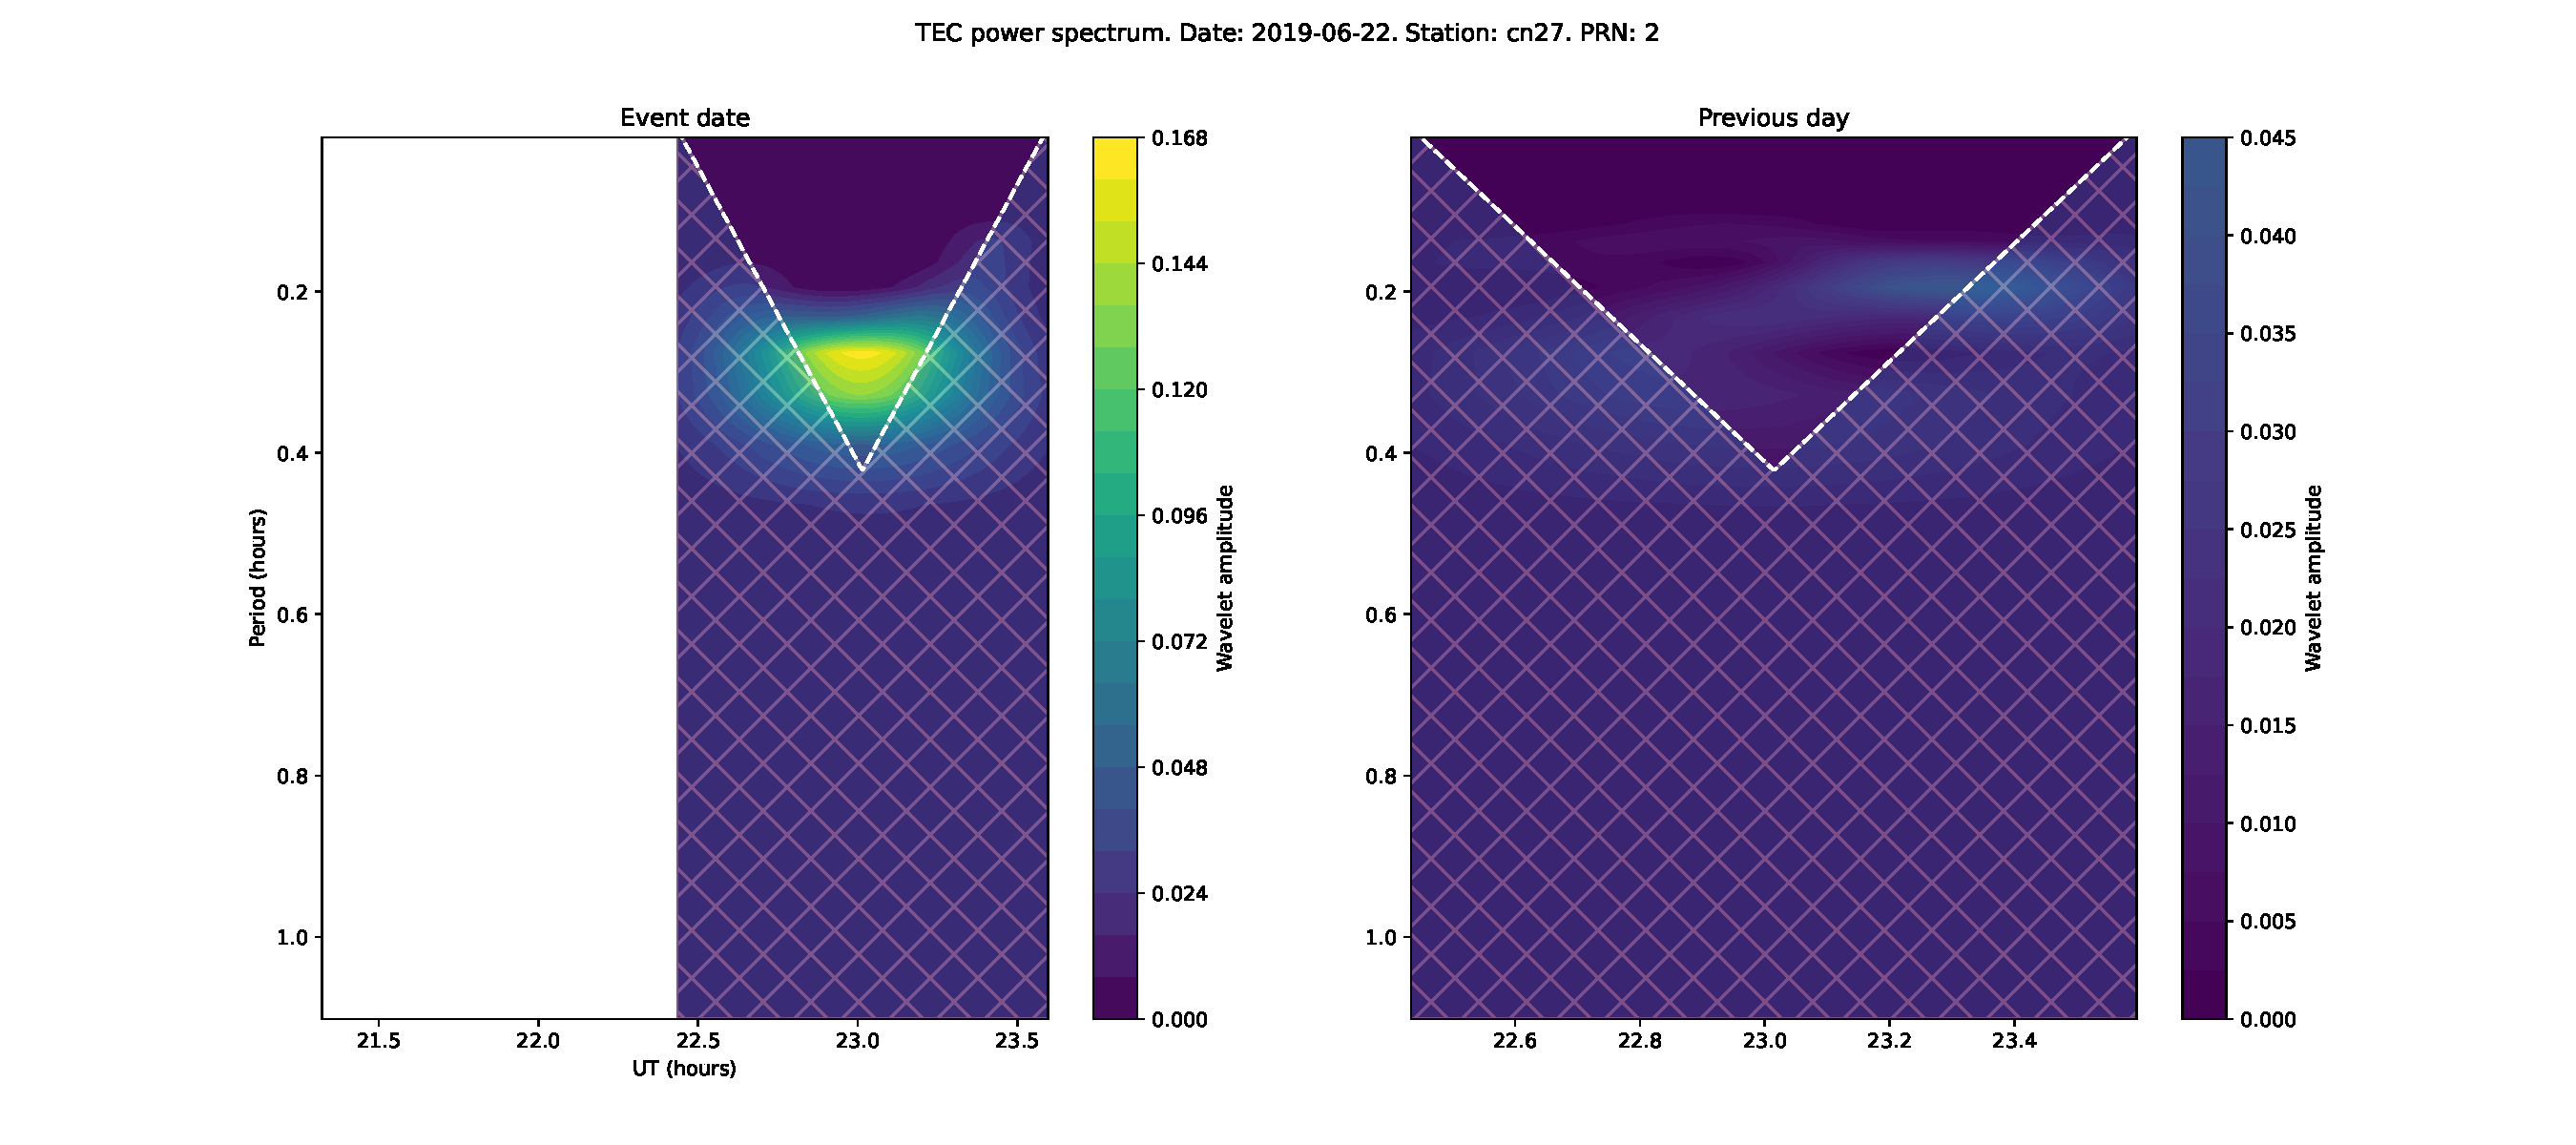
\includegraphics[width=0.5\linewidth]{./figures/cn27-PRN2-contour}\\
%  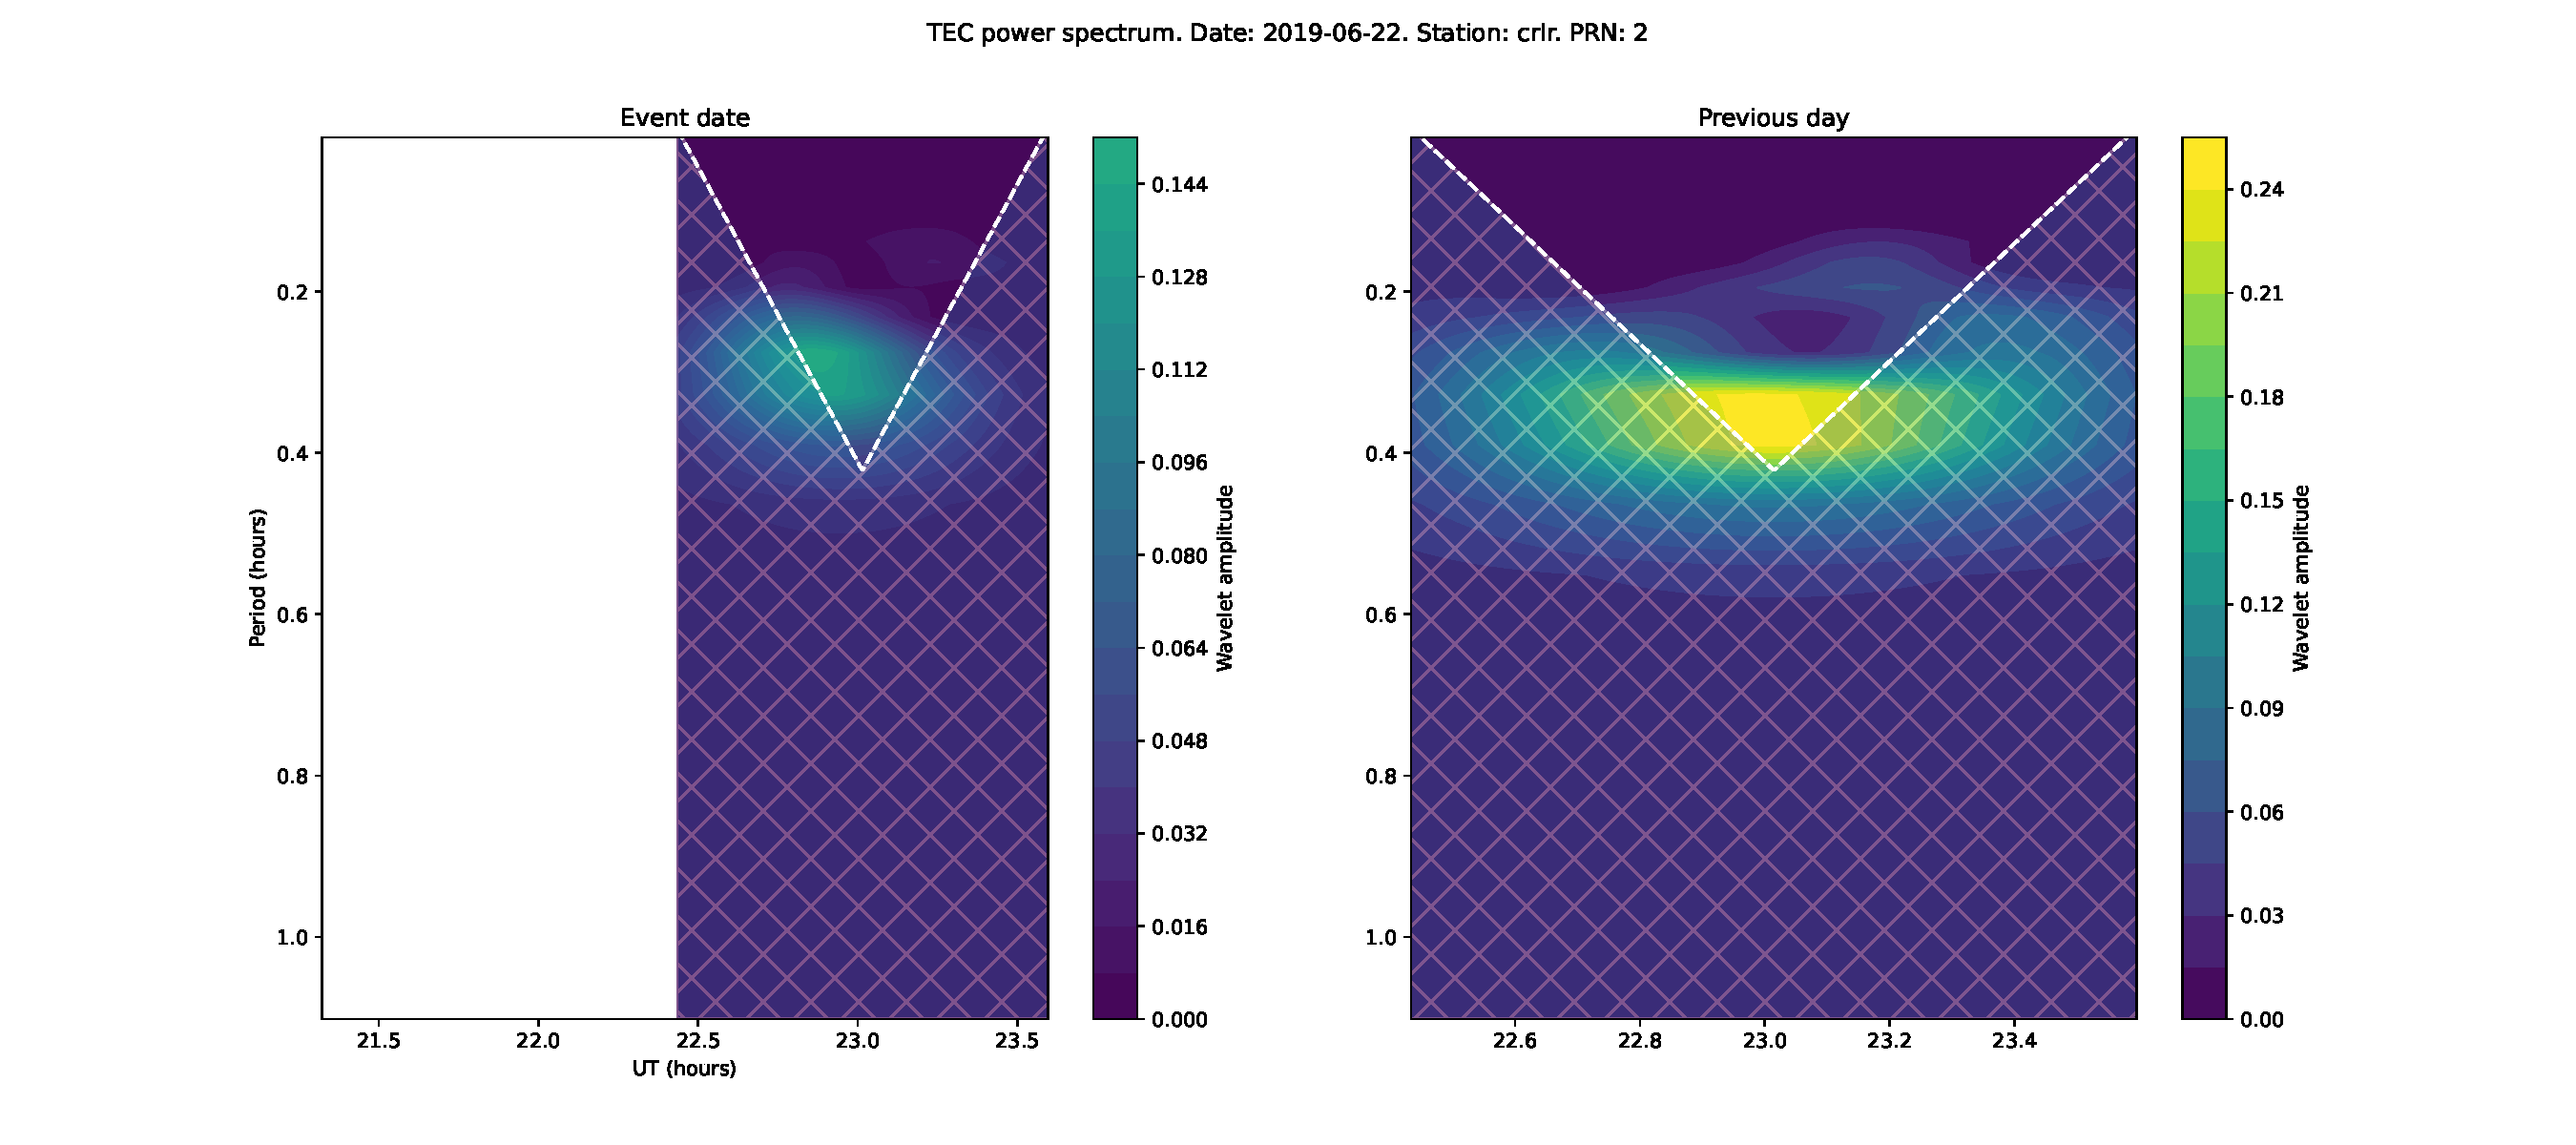
\includegraphics[width=0.5\linewidth]{./figures/crlr-PRN2-contour}  & %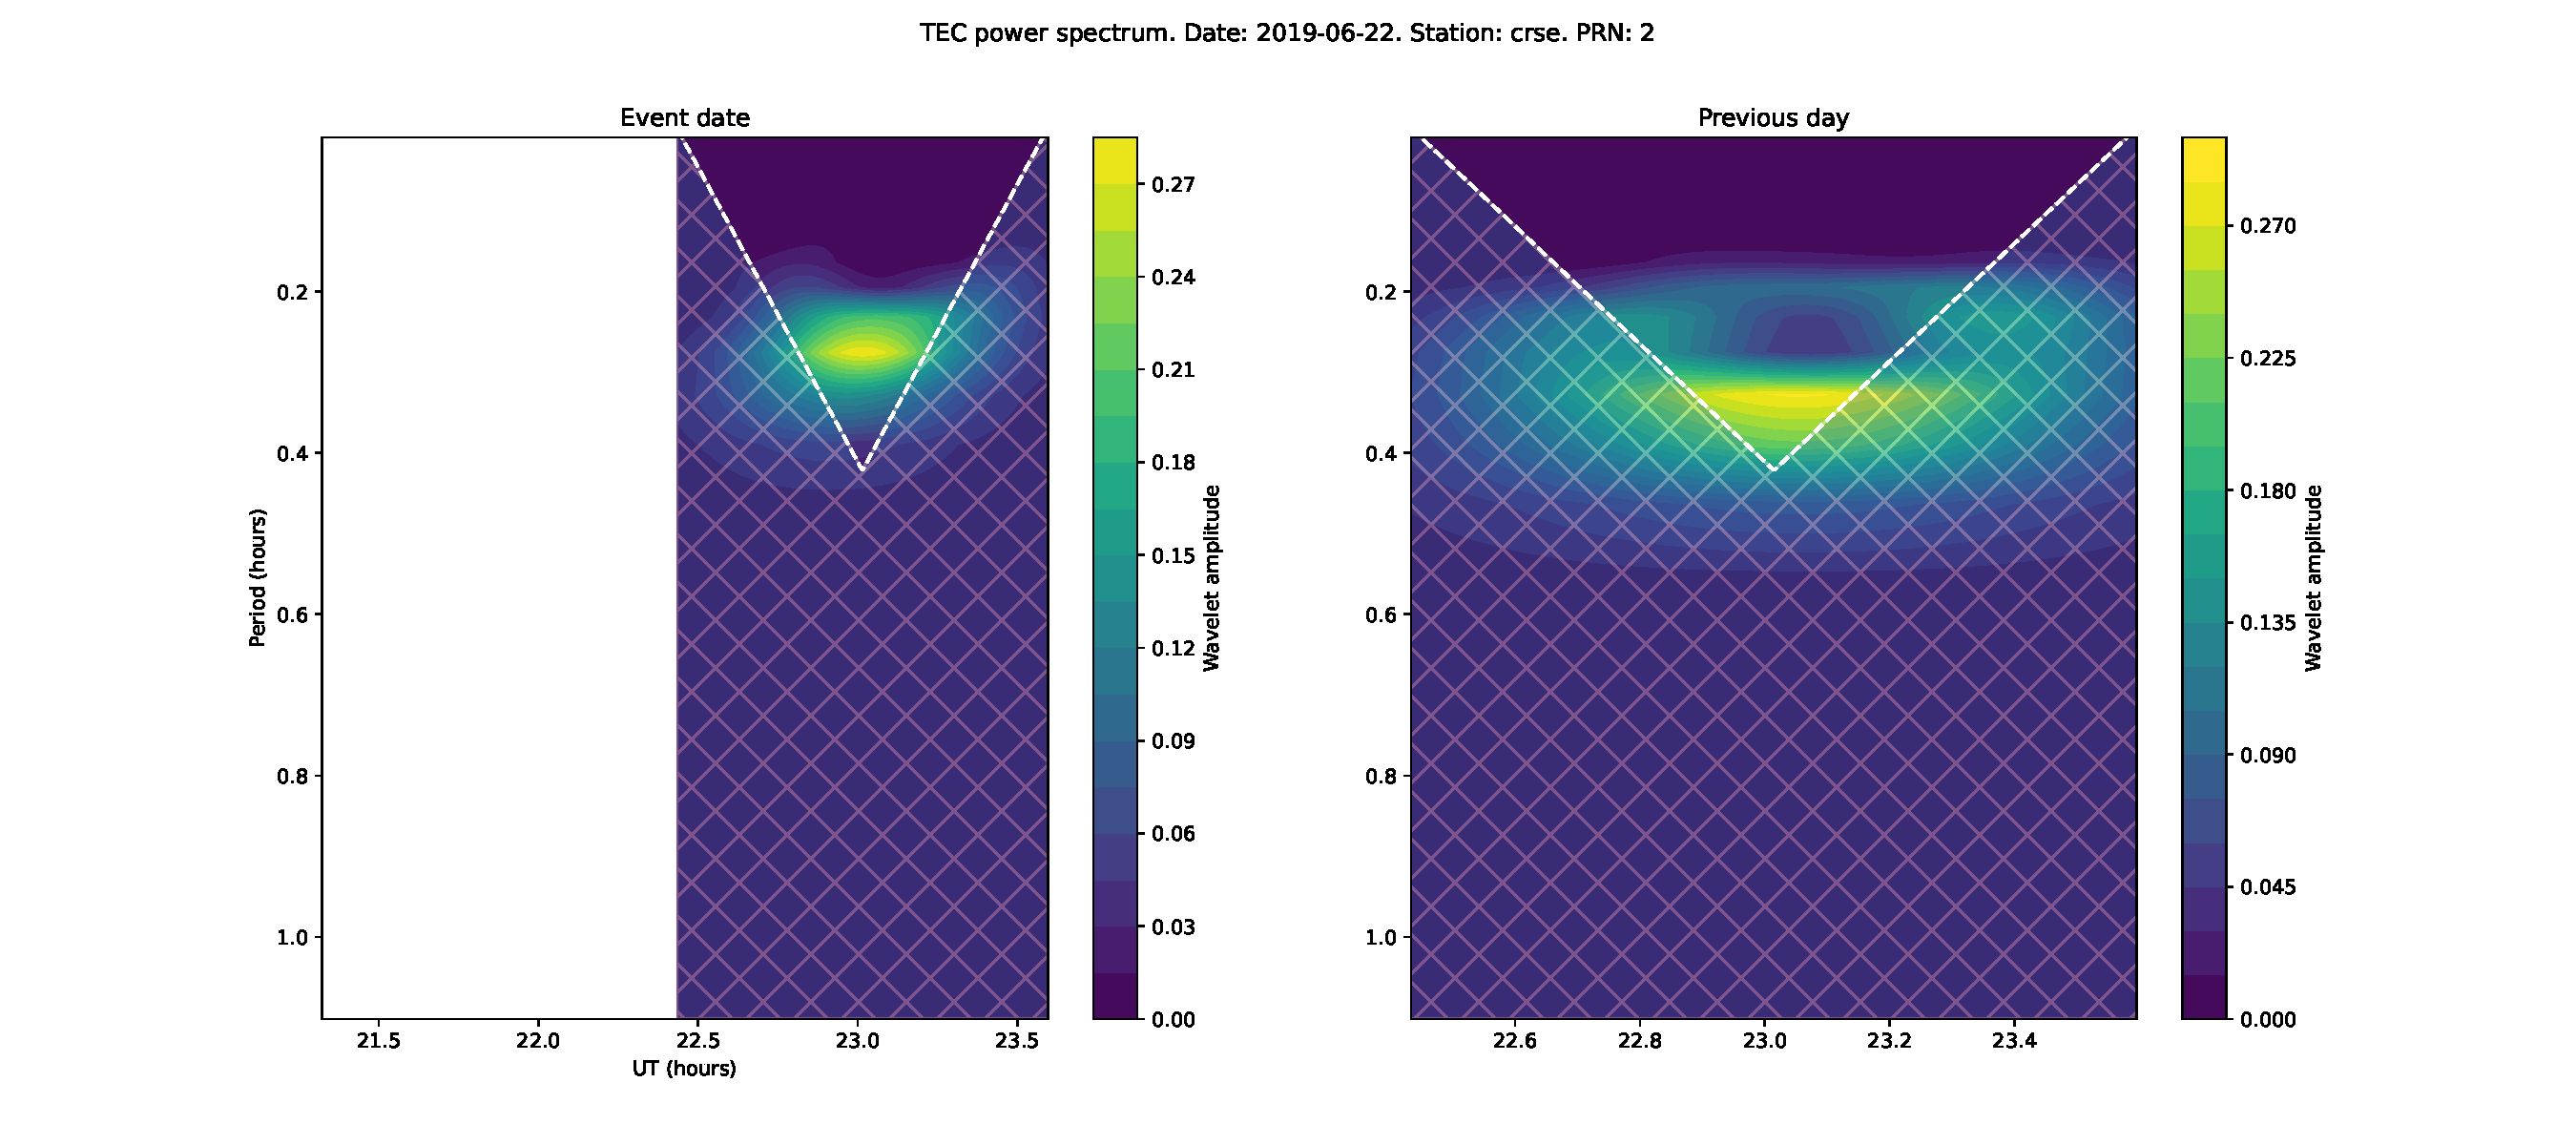
\includegraphics[width=0.5\linewidth]{./figures/crse-PRN2-contour}
%  \end{tabular}
%  \label{fig:power-spectrums}
%  \caption{Examples of power spectrums for event USG-09, PRN 2. Top left: Station CN05. Top Right: Station CN27. Bottom left: station CRLR. Bottom right: station CRSE. In each figure the left panel corresponds to the event day and the right panel corresponds to the previous day of the event. The white dashed lines correspond to the Cone of Influence, where all the wavelet spectrum below is subject to error.}
%\end{figure*}

  